\documentclass[a4paper, 1.5lines]{ctexart}
\usepackage[top=3cm, bottom=2cm]{geometry}
\usepackage{graphicx}
\usepackage{subcaption}
\usepackage{amsmath}
\usepackage{amssymb}
\usepackage{xcolor}
\usepackage{url}
\usepackage{booktabs}
\usepackage{multirow}
%\usepackage{hyperref}
\usepackage[hidelinks]{hyperref} % 加载 hyperref 并隐藏链接边框

%\usepackage[utf8]{inputenc}
%\usepackage[ngerman]{babel} % 加载德语支持

% booktabs 提供 \toprule, \midrule, \bottomrule 等表格命令
\usepackage{booktabs}
% 定义占位命令以避免未定义控制序列错误
\newcommand{\placeholderspace}{}
\usepackage{fancyhdr} % 导入fancyhdr宏包
\usepackage{lipsum}   % 仅用于生成示例文本
\usepackage{float}    % 提供 H 浮动位置选项

% 设置页面样式为fancy
\pagestyle{fancy}
% 自定义页眉内容
\fancyhead[L]{} % 左侧页眉
\fancyhead[C]{\textbf{Physics-experiment Reporting Letter:\\Magnetron Sputtering Coating Technology}} % 中间页眉
\fancyhead[R]{ } % 右侧页眉
% 自定义页脚内容
\fancyfoot[L]{ } % 左侧页脚
\fancyfoot[C]{\thepage} % 中间页脚显示页码
\fancyfoot[R]{ } % 右侧页脚
% 改变页眉线的粗细
\renewcommand{\headrulewidth}{1.4pt}
% 改变页脚线的粗细
\renewcommand{\footrulewidth}{0.pt}





\title{磁控溅射镀膜技术}
\author{实验人：学生\qquad 学号：[学号已脱敏]\qquad 指导教师：王海波}
\date{实验日期：2026.4.3}


\begin{document}
    
    \maketitle
    
    \begin{abstract}
         本实验旨在研究磁控溅射镀膜技术的基本原理及其应用。实验采用直流磁控溅射方法制备金属 Cu 薄膜，并通过膜厚测量与电学测试等手段对薄膜性质进行表征。实验结果表明，在适当的放电条件与气压范围下可以获得连续且稳定的金属薄膜。与体材料相比，所制备薄膜的电阻率明显偏大，反映出薄膜中存在缺陷、晶界散射及结构不均匀性等因素的影响。此外，形貌测试结果显示薄膜表面具有一定程度的非均匀性。这些结果表明，磁控溅射工艺参数对薄膜质量具有重要影响。\\
    \textbf{\textbf{关键词：磁控溅射 \quad 台阶仪 \quad 四引线法 \quad 薄膜电阻率}}
    \end{abstract}
    
    \section{引言}
    在薄膜材料制备技术的发展过程中，磁控溅射作为一种重要的物理气相沉积方法，因其成膜均匀性好、可控性强以及适用材料范围广等优点，被广泛应用于微电子器件、光学薄膜及功能材料等领域。该技术通过在低压气体环境中引入电场与磁场，使气体发生辉光放电并形成等离子体，高能离子轰击靶材表面，从而将靶材原子溅射出来并沉积在基底上形成薄膜。

    在这一过程中，真空环境的建立是实现稳定放电与高质量成膜的前提。气体放电产生的等离子体中包含大量电子与离子，它们在电磁场作用下发生复杂运动，并不断与靶材发生相互作用，将动能传递给靶材原子，实现材料的溅射与迁移。与此同时，溅射粒子在基底表面的扩散、吸附及再排列过程，又进一步决定了薄膜的结构与性能。

    通过调节工作气压、放电功率以及磁场分布等实验参数，可以有效控制等离子体特性及溅射过程，从而影响薄膜的沉积速率、致密性与电学性质。因此，磁控溅射过程本质上是一个涉及等离子体物理、表面物理及材料科学的多物理场耦合过程。

    本实验以金属 Cu 薄膜的制备为例，通过实际操作磁控溅射装置，观察放电现象并调控实验参数，同时结合膜厚与电学测量结果，对薄膜的基本性质进行分析，从而加深对磁控溅射镀膜机理及其工艺特性的理解。

    \section{原理}
        \subsection{气体辉光放电与等离子体形成}

在磁控溅射过程中，首先需要将系统抽至高真空状态（约 $10^{-5}\sim10^{-4}$ Pa），以减少杂质气体对放电过程及薄膜质量的影响。随后引入惰性气体（通常为 Ar）作为工作气体。

当在电极之间施加电压时，气体中的少量自由电子在电场作用下被加速，与中性气体原子发生碰撞并引发电离，从而产生更多电子与离子，形成电子雪崩过程。随着电压进一步升高，气体放电由汤生放电逐渐过渡到辉光放电状态。在稳定辉光放电条件下，系统中形成由电子、离子及中性粒子组成的等离子体体系，其整体呈电中性，但具有良好的导电性与较高的粒子活性。

\subsection{溅射过程}

在等离子体中，正离子（主要为 Ar$^+$）在电场作用下加速并轰击靶材表面，将动能传递给靶原子。当入射离子的能量超过表面束缚能时，靶材原子将被击出并进入气相，该过程称为溅射。

溅射效率通常用溅射产额表征，其定义为单位入射离子所对应溅射出的原子数。溅射产额与入射离子的能量、入射角以及靶材的原子结构密切相关。一般而言，入射能量越高，溅射产额越大，但当能量过高时也可能引入不稳定因素。

\subsection{薄膜的形成机制}

被溅射出的原子在真空环境中传播并最终沉积到基底表面。到达基底后，这些原子经历吸附、表面扩散、成核以及长大等过程，逐渐形成连续薄膜。

根据原子与基底之间相互作用强度的不同，薄膜的生长模式通常可分为三类：岛状生长（Volmer-Weber 模式）、层状生长（Frank-van der Merwe 模式）以及层岛混合生长（Stranski-Krastanov 模式）。不同生长模式会显著影响薄膜的微观结构、表面粗糙度及附着性能。

\begin{figure}[h!]
    \centering
    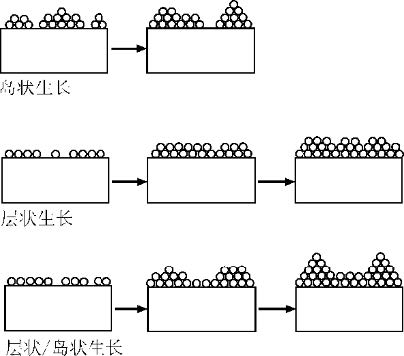
\includegraphics[width=0.75\textwidth]{fig//grow}
    \caption{薄膜生长模式示意图}
    \label{fig:grow}
\end{figure}


\subsection{真空系统与抽气方法}

为了获得稳定的放电条件与良好的薄膜质量，需要建立高真空环境。本实验采用机械泵与涡轮分子泵的组合抽气方式。

首先利用机械泵将系统抽至低真空区（约 $10^{-1}$ Pa），随后启动涡轮分子泵，将压强进一步降低至高真空范围（$10^{-5}\sim10^{-4}$ Pa）。该两级抽气方式既保证了抽气效率，又能够有效覆盖不同压强范围。

\subsection{真空度的测量}

实验中采用复合真空计对系统压强进行测量，包括热偶真空计与电离真空计两种类型。

\begin{itemize}
    \item \textbf{热偶真空计}：适用于低真空区域（约 $10^{1}\sim10^{-1}$ Pa），其工作原理基于气体热导率随压强变化的特性。
    \item \textbf{电离真空计}：适用于高真空区域（约 $10^{-1}\sim10^{-5}$ Pa），通过气体电离产生的离子电流来反映压强大小。需要注意的是，只有在压强低于约 $10^{-1}$ Pa 时才能开启电离规，以避免损坏仪器。
\end{itemize}

\subsection{薄膜表征方法}

薄膜的结构与性能需要通过多种实验手段进行综合表征。本实验主要采用石英晶体振荡法、台阶仪法以及四探针法。

\begin{itemize}
    \item \textbf{石英晶体振荡法}：利用石英晶体振荡频率随质量变化的关系，实现对薄膜沉积厚度的高精度测量。
    \item \textbf{台阶仪法}：通过测量薄膜与基底之间的台阶高度来获得膜厚信息，该方法直观但属于接触式测量。
    \item \textbf{四探针法}：用于测量薄膜的电阻率，能够有效减小接触电阻对测量结果的影响，适用于均匀薄膜体系。
\end{itemize}

\subsection{磁控溅射技术特点}

根据供电方式与工作机制的不同，溅射技术可分为直流溅射、射频溅射及磁控溅射等类型。

磁控溅射在靶材附近引入磁场，使电子在局部区域内作回旋运动，从而显著延长其运动路径，提高电离效率。这不仅增强了等离子体密度，也提高了溅射沉积速率。同时，由于工作气压可以降低，薄膜纯度与致密性也得到改善。

此外，通过引入反应气体，还可实现反应溅射，从而制备氧化物或氮化物等功能薄膜材料。

    \section{实验}
    
        \subsection{直流溅射制备 Cu 薄膜}

\begin{enumerate}
    \item \textbf{基片准备与装载} \\
    对基片进行超声清洗以去除表面污染物，干燥后固定于样品托盘，并将托盘放入真空腔体中。

    \item \textbf{抽真空与气氛建立} \\
    按照操作规程启动真空系统，先由机械泵抽至低真空，再由分子泵抽至高真空（约 $10^{-5}\sim10^{-4}$ Pa）。当真空度达到要求后关闭电离规，通入工作气体 Ar，并通过质量流量控制器（MFC）调节气体流量，使腔体压强稳定在设定值。

    \item \textbf{放电与溅射沉积} \\
    打开直流溅射电源，逐步调节电压与电流至稳定辉光放电状态。在稳定放电条件下进行溅射沉积，沉积时间约为 $30\ \text{min}$。实验过程中控制工作气压与输入功率
    ，并记录薄膜生长速率等相关参数。

    \item \textbf{关机与样品取出} \\
    溅射结束后关闭电源，继续抽真空以排除残余气体，随后按照操作规程逐步关机并取出样品。
\end{enumerate}

\subsection{样品表征方法}

\begin{itemize}
    \item \textbf{膜厚测量} \\
    利用台阶仪测量薄膜厚度 $d$，并与原位膜厚监测结果进行对比，以评估沉积速率及测量一致性。

    \item \textbf{电学性能测量} \\
    采用范德堡法测量薄膜的电阻率 $\rho$，并与体材料的理论值进行比较，从而分析薄膜中晶界散射、缺陷及结构不均匀性等因素对电学性能的影响。
\end{itemize}

    \section{结果与分析讨论}
    
        \subsection{台阶仪测量 Cu 薄膜厚度}

在镀膜过程中，当沉积时间达到 $t = 30\mathrm{min}49\mathrm{s}$ 时停止溅射。此时原位石英晶体膜厚监测仪显示膜厚约为 $d_{\text{monitor}} = 2000\text{\AA}$，时厚$380\text{\AA}$，对应沉积速率约为 $0.19\mathrm{\text{\AA}/s}$。实验过程中腔体压强稳定在 $p \approx 0.6\mathrm{Pa}$，环境温度约为 $T \sim 21\mathrm{^\circ C}$。

将样品取出后，利用台阶仪对薄膜厚度进行测量。通过改变样品摆放方式，在不同位置进行多次测量，结果如图\ref{fig:step_results}所示。可以得到薄膜厚度的平均值为
\begin{equation}
    \bar{d} = 3308.5\ \text{\AA}
\end{equation}

\begin{figure}[h!]
    \centering
    
    \begin{subfigure}{0.45\textwidth}
        \centering
        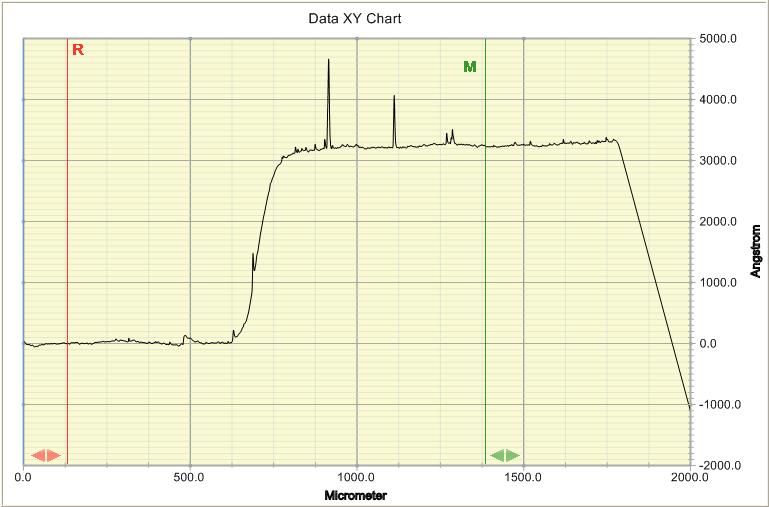
\includegraphics[width=\textwidth]{fig/1}
        \caption{台阶仪测量结果1}
        \label{fig:step_cross}
    \end{subfigure}
    \hfill
    \begin{subfigure}{0.45\textwidth}
        \centering
        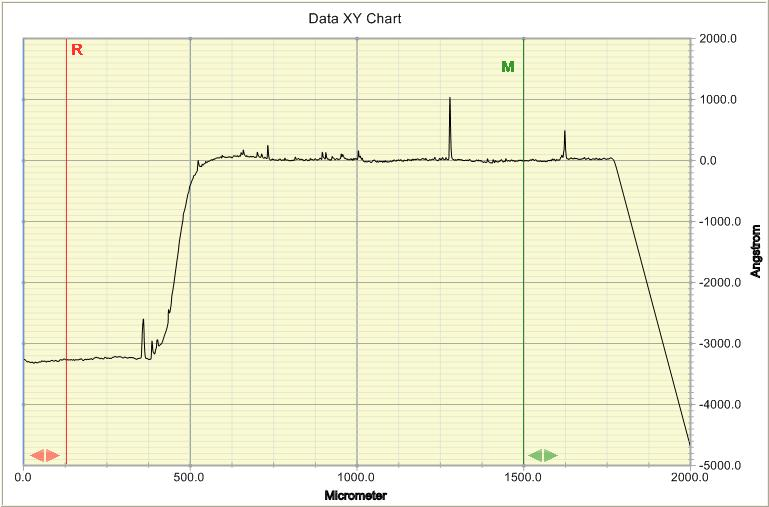
\includegraphics[width=\textwidth]{fig/2}
        \caption{台阶仪测量结果2}
        \label{fig:step_instrument}
    \end{subfigure}

    \vspace{0.5em}

    \begin{subfigure}{0.45\textwidth}
        \centering
        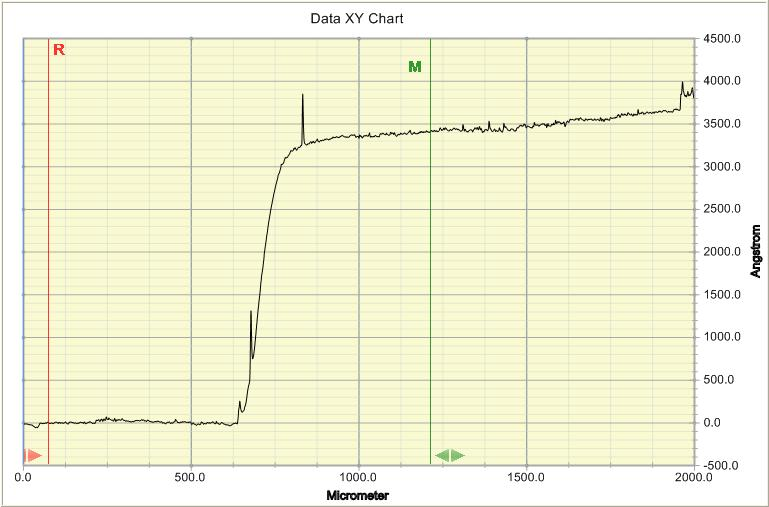
\includegraphics[width=\textwidth]{fig/3}
        \caption{台阶仪测量结果3}
        \label{fig:step_film}
    \end{subfigure}

    \caption{台阶仪测量结果示例}
    \label{fig:step_results}
\end{figure}

从台阶仪扫描结果可以观察到以下特征：

首先，在跨越“有膜/无膜”区域的扫描中，可以清晰识别出膜层台阶，表明薄膜沉积成功。同时，在有膜区域内部，膜厚呈现一定的空间变化趋势，即不同位置的膜厚存在差异。

其次，在仅扫描有膜区域时，测得表面起伏较为明显，局部高度变化可达数百 \AA 量级。这说明薄膜表面存在较强的粗糙度。

上述现象可以从薄膜生长机制加以理解。对于金属薄膜，在一定条件下更倾向于岛状（Volmer-Weber）生长模式，即原子在基底表面优先形成局域岛状结构，随后逐渐并合形成连续膜层。在该过程中，不同区域的成核密度及生长速率存在差异，从而导致膜厚不均匀及表面起伏。

此外，基底表面状态（如是否覆盖胶带）也可能影响局部成核行为，从而导致膜厚在空间上的非均匀分布。

另一方面，测量结果中的局部尖峰与起伏还可能受到以下因素影响：一是薄膜本身的表面粗糙度；二是台阶仪探针在扫描过程中对微观结构的响应；三是环境振动或仪器稳定性对测量信号的扰动。

最后，对比原位膜厚仪与台阶仪的测量结果可以发现二者存在一定差异。这主要是由于两种测量方法的物理机制不同：石英晶体振荡法测量的是参考位置处的沉积质量变化，而台阶仪测量的是实际样品表面的几何厚度。由于沉积过程中空间分布不完全均匀，两者结果存在偏差是合理的。


\subsection{范德堡法测量 Cu 薄膜电阻率}

采用范德堡法对薄膜电阻率进行测量，得到多组实验数据，并绘制其统计分布，如图\ref{fig:multiexp}所示。

\begin{figure}[h!]
    \centering
    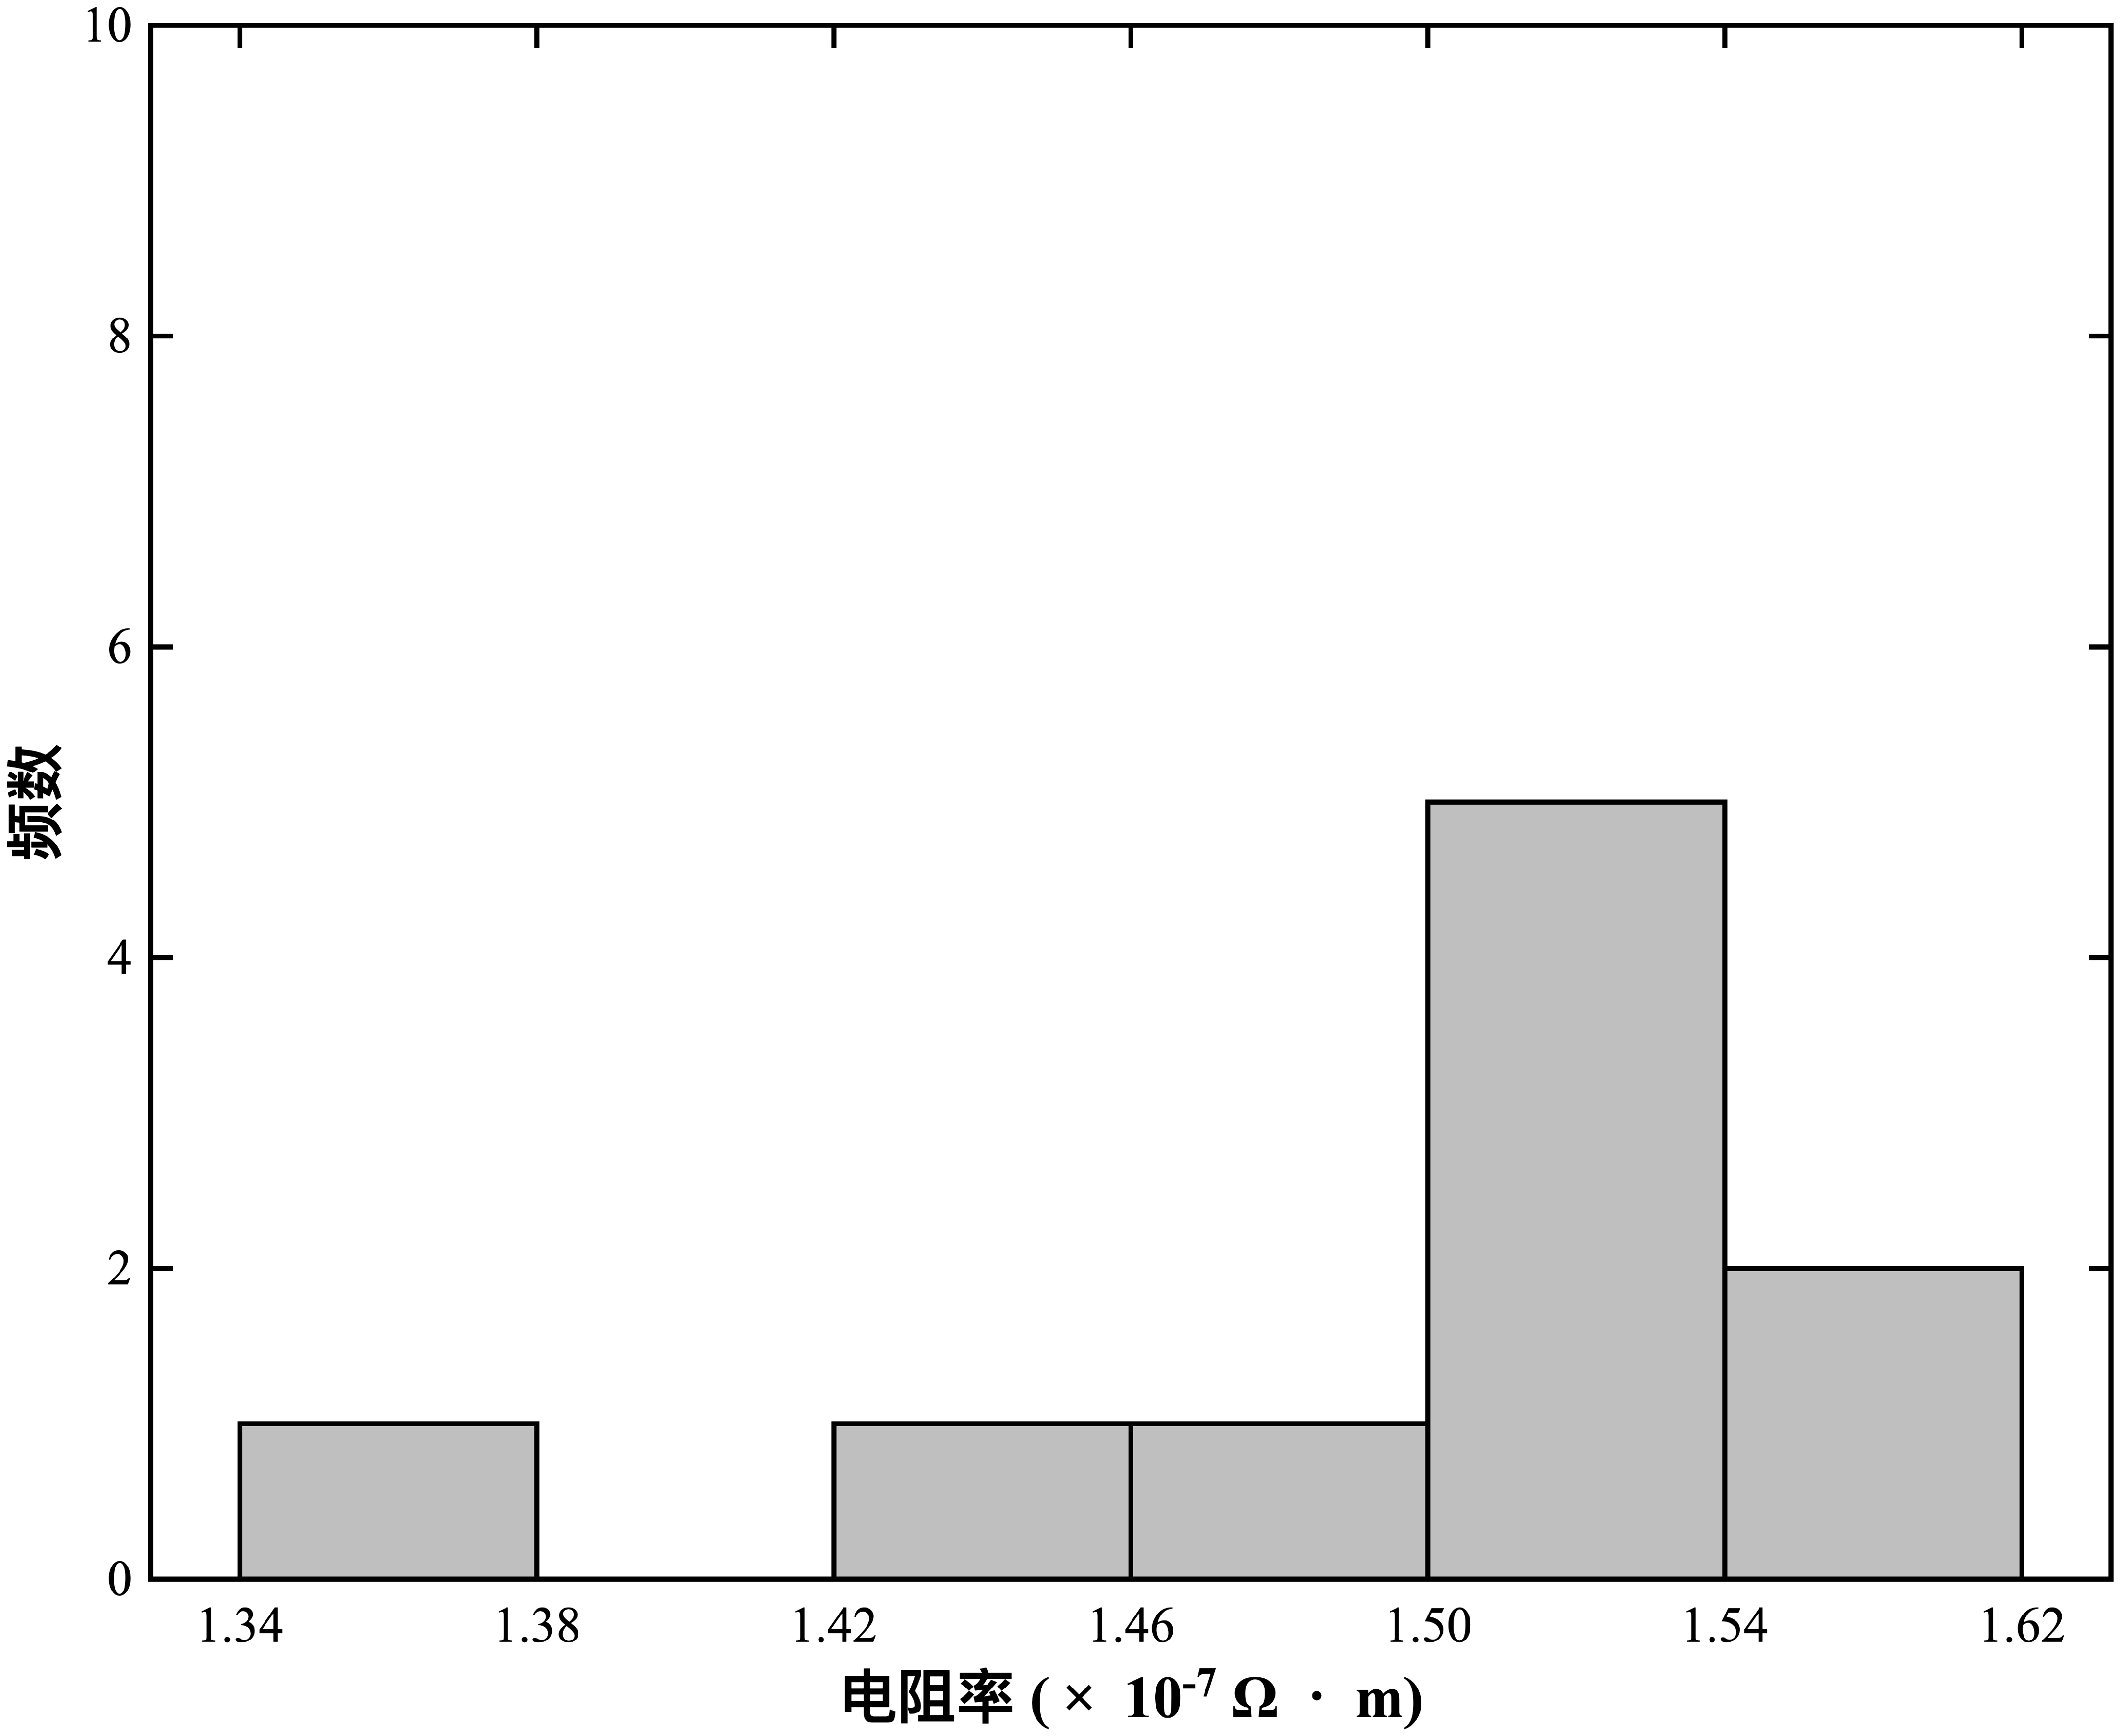
\includegraphics[width=0.75\textwidth]{fig//his}
    \caption{电阻率数据分布}
    \label{fig:multiexp}
\end{figure}

对测量结果取平均，得到薄膜电阻率为
\begin{equation}
    \rho = 1.511 \times 10^{-7}\ \Omega \cdot \text{m}
\end{equation}

查阅文献可知，块体 Cu 的电阻率约为
\begin{equation}
    \rho_{\text{bulk}} = 1.678 \times 10^{-8}\ \Omega \cdot \text{m}
\end{equation}

可以看到，薄膜的电阻率显著高于块体材料，其主要原因包括：

首先，薄膜中存在大量晶界与缺陷结构，这些结构会增强电子散射，从而降低载流子迁移率；

其次，薄膜厚度较小，表面散射效应显著，电子在传输过程中更容易与界面发生相互作用；

此外，沉积过程中引入的杂质或非理想结构也可能对电学性能产生影响。

总体而言，实验结果与薄膜物理中关于尺寸效应与缺陷散射的理论预期相一致。
    \section{总结}

    本次实验成功地运用了磁控溅射镀膜技术制备了金属 Cu 薄膜，并对其性能进行了较为系统的分析。实验过程中，通过机械泵与涡轮分子泵的组合实现了所需的高真空环境，并在特定放电条件下完成了 Cu 膜的稳定沉积。通过对样品的测量可以发现，尽管大部分区域内薄膜厚度相对一致，但局部区域仍表现出一定的厚度差异及表面粗糙度。这一现象可能与靶材原子在衬底及胶带区域的沉积行为差异有关，同时实验环境扰动及仪器稳定性也可能对测量结果产生影响。

另一方面，实验测得的 Cu 薄膜电阻率与块体材料相比存在一定偏差。结合实验过程分析，该偏差更可能来源于测量过程中的系统误差，例如膜厚测量的不确定性、范德堡法对样品几何条件的理想假设未完全满足，以及电极接触等因素的影响，而不完全反映材料本征电学性质的变化。

为进一步分析 Cu 薄膜的性能，可以在后续实验中扩大台阶仪的扫描范围，对薄膜表面形貌进行更全面的统计分析，以判断不均匀性是否与岛状生长模式相关。此外，还可以结合膜厚分布与电阻率测量结果进行对比分析，从而探究薄膜结构与电学性质之间的潜在关联。
    \begin{thebibliography}{99}
        \bibitem{1}
        北京师范大学物理实验教学中心. 近代物理实验讲义一 (2019)
    \end{thebibliography}

    \newpage
    \section*{附录：原始数据图}

\begin{figure}[H]
    \centering

    \begin{subfigure}{0.75\textwidth}
        \includegraphics[width=\textwidth]{fig/origin_data_1}
        \caption{原始数据1}
    \end{subfigure}

    \vspace{0.5em}

    \begin{subfigure}{0.75\textwidth}
        \includegraphics[width=\textwidth]{fig/origin_data_2}
        \caption{原始数据2}
    \end{subfigure}

    \caption{实验原始数据（1）}
\end{figure}

\begin{figure}[H]
    \centering

    \begin{subfigure}{0.75\textwidth}
        \includegraphics[width=\textwidth]{fig/origin_data_3}
        \caption{原始数据3}
    \end{subfigure}

    \vspace{0.5em}

    \begin{subfigure}{0.75\textwidth}
        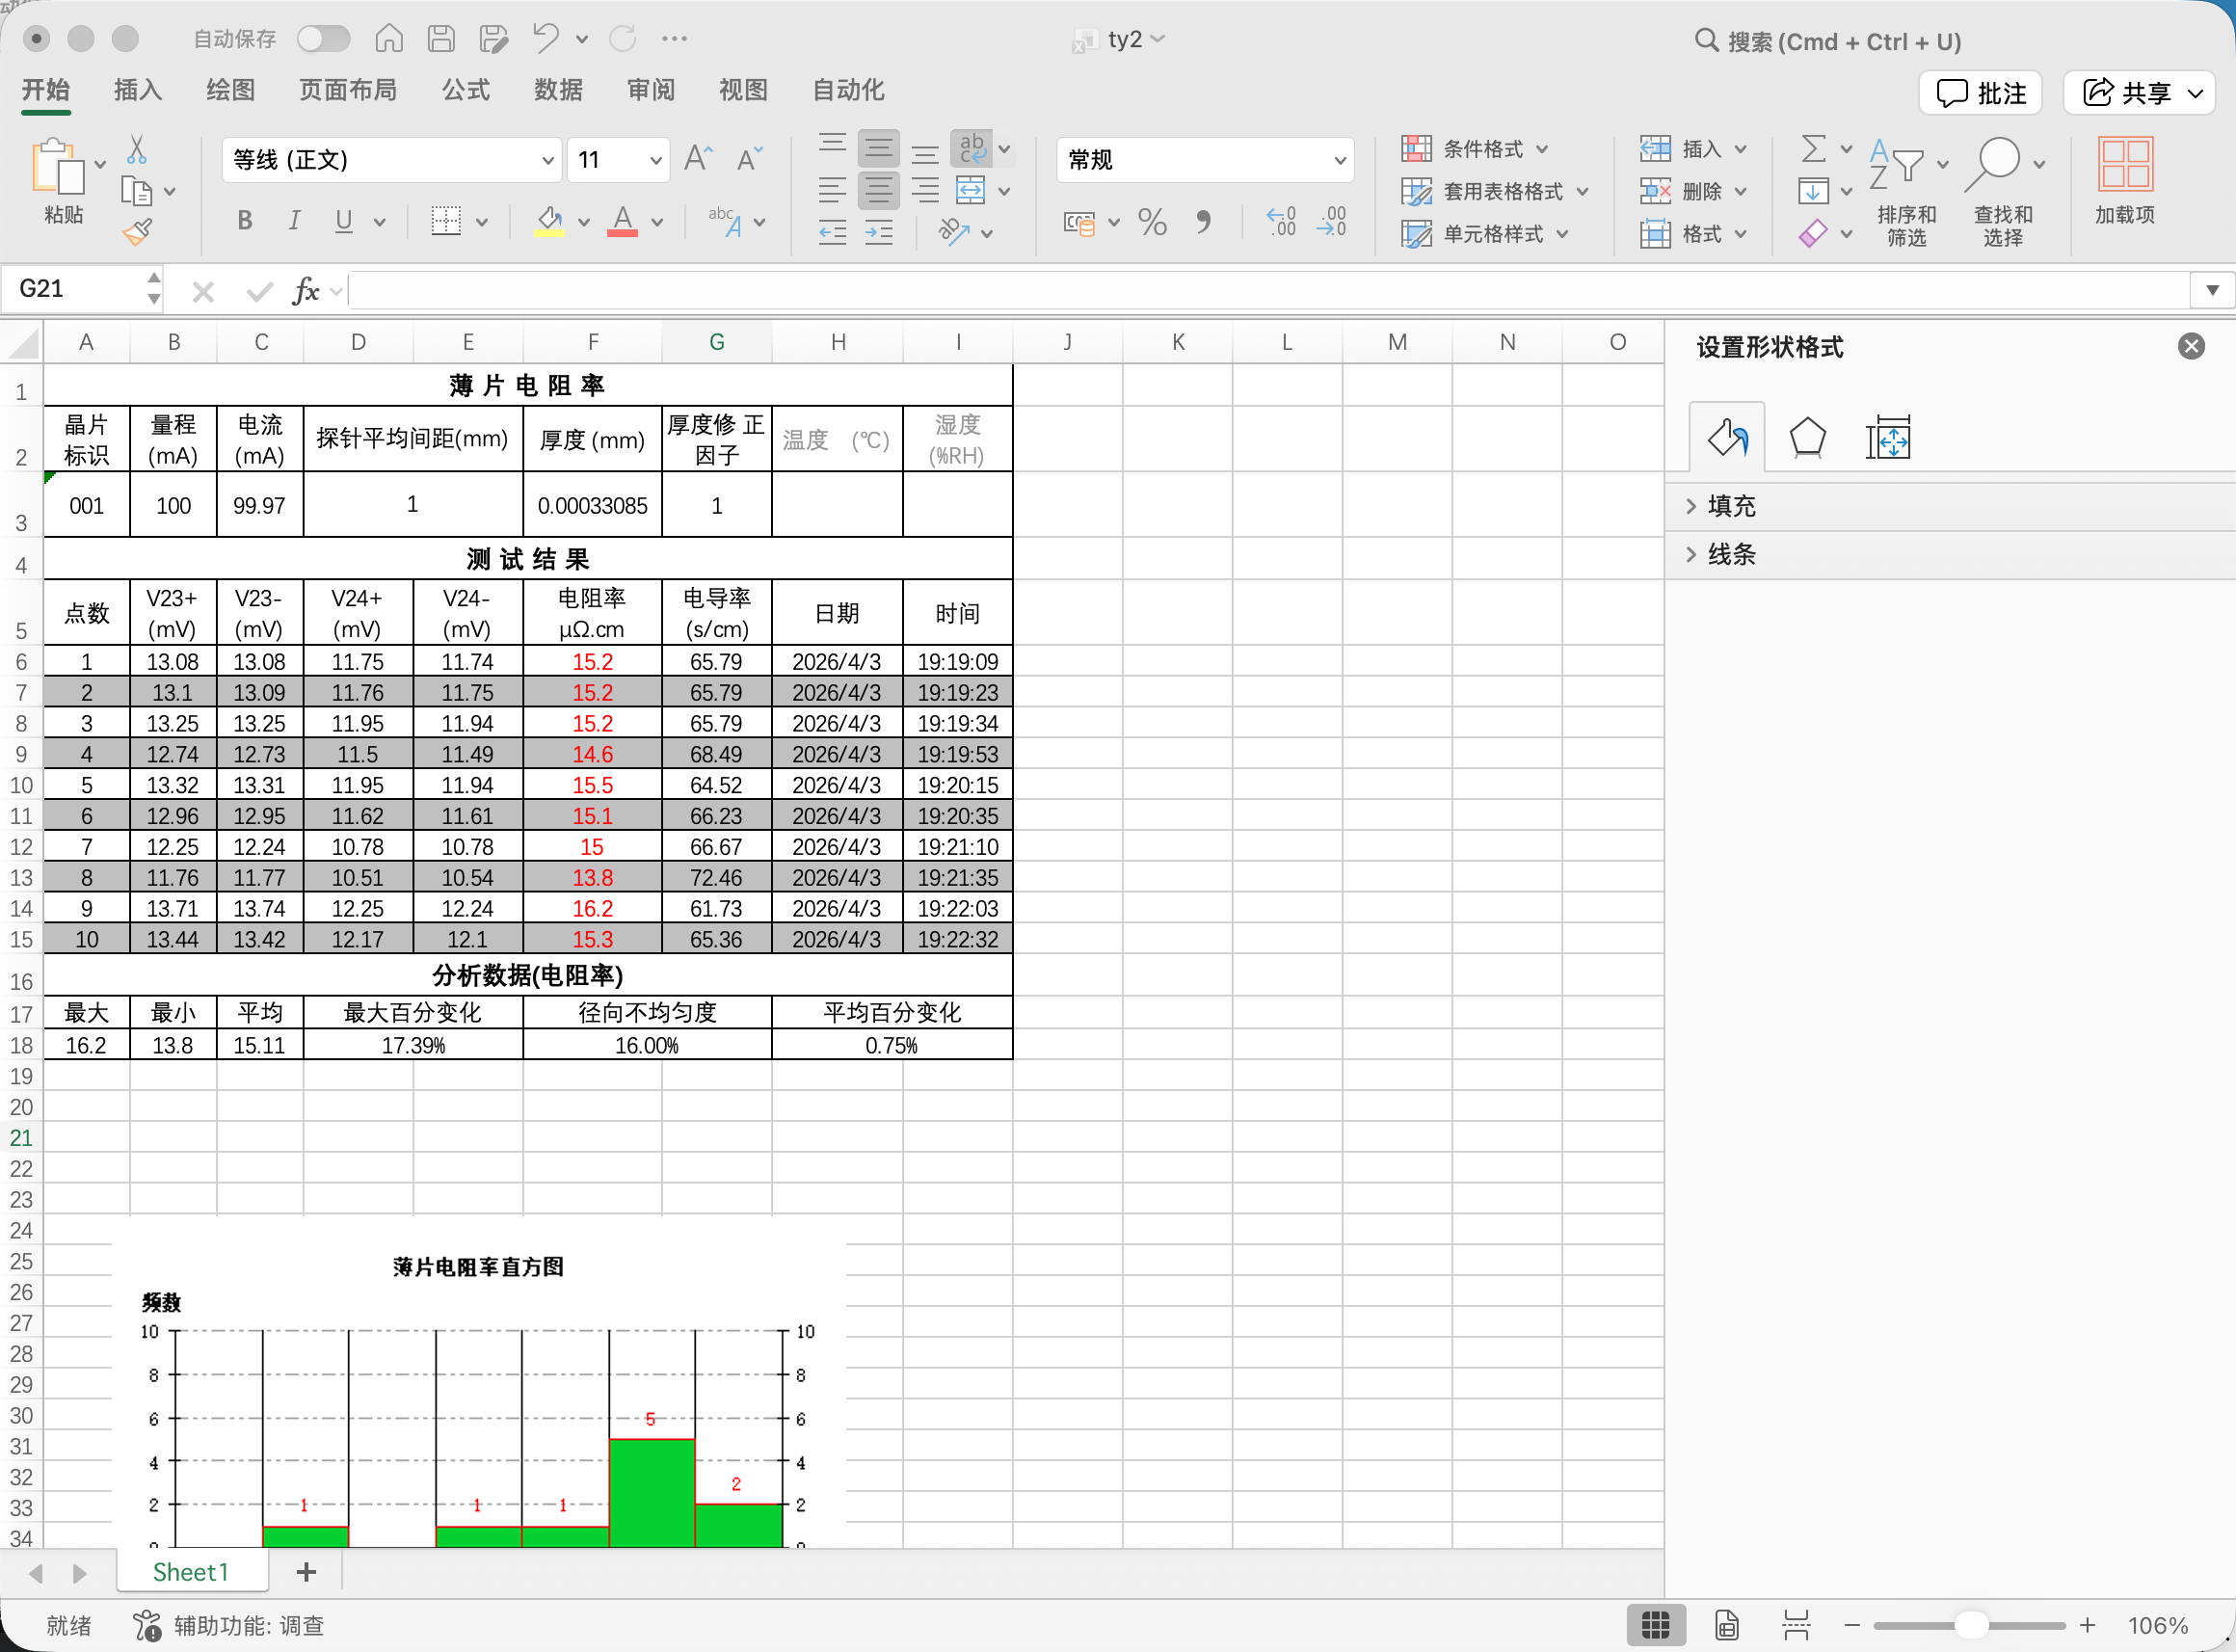
\includegraphics[width=\textwidth]{fig/origin_data_4}
        \caption{原始数据4}
    \end{subfigure}

    \caption{实验原始数据（2）}
\end{figure}



\end{document}